\documentclass{article}
\usepackage{tikz}
\usepackage{amsmath}
\usetikzlibrary{shapes.geometric, arrows}

\tikzstyle{startstop} = [rectangle, rounded corners, minimum width=3cm, minimum height=1cm,text centered, draw=black, fill=red!30]
\tikzstyle{process} = [rectangle, minimum width=3cm, minimum height=1cm, text centered, draw=black, fill=blue!30]
\tikzstyle{decision} = [diamond, minimum width=3cm, minimum height=1cm, text centered, draw=black, fill=green!30]
\tikzstyle{arrow} = [thick,->,>=stealth]

\begin{document}


\section{Pipeline Overview}
We have a list of unreviewed claims paired with reviewed claims, each labeled with $0$ or $1$ to indicate whether they are similar or not. Using this dataset, we train a binary classifier with a large language model (LLM) to determine whether an unreviewed claim is similar to another.

The pipeline consists of the following steps:
\begin{enumerate}
    \item \textbf{Ranking System:} The process starts with a ranking system that identifies the top $K$ reviewed claims most similar to the input unreviewed claim. This is achieved by leveraging a transformer model to compute similarities between the unreviewed claim and all reviewed claims, selecting the top $K$ based on similarity scores.
    \item \textbf{Binary Classification for Re-Ranking:} The top $K$ claims are then passed through a binary classifier that acts as a re-ranking step. This classifier filters out claims from the top $K$ list that are not sufficiently similar, according to the binary classification model.
    \item \textbf{Final Selection:} After re-ranking, the claims retained by the classifier are presented as the final output. These claims represent the reviewed claims deemed most similar to the input unreviewed claim.
\end{enumerate}



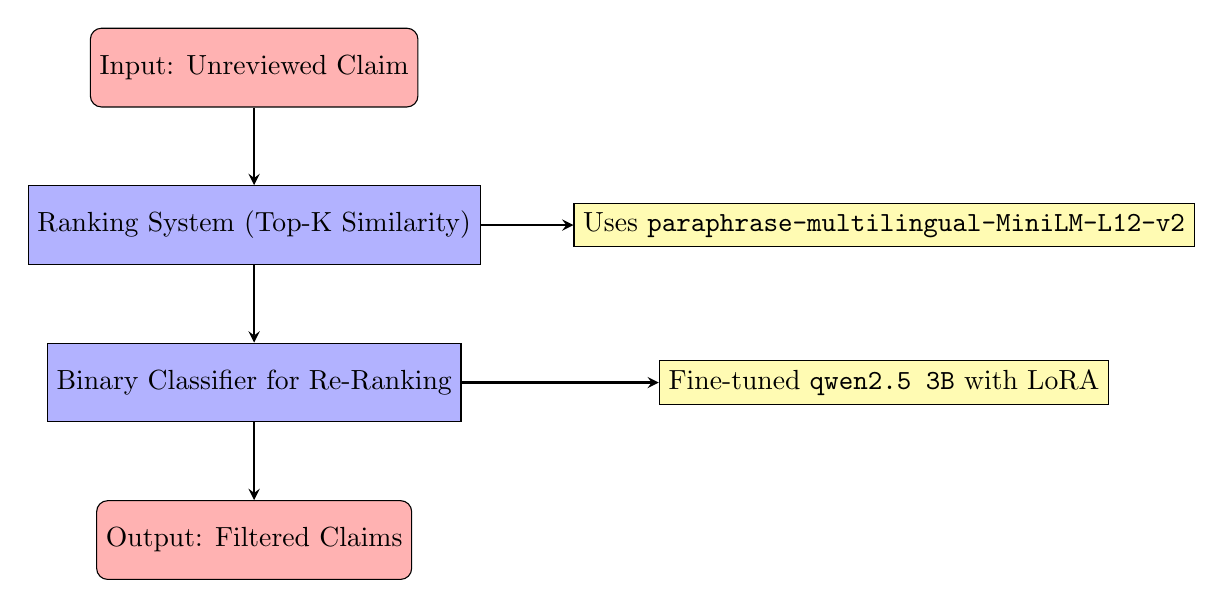
\begin{tikzpicture}[node distance=2cm]

\node (start) [startstop] {Input: Unreviewed Claim};
\node (ranking) [process, below of=start] {Ranking System (Top-K Similarity)};
\node (rerank) [process, below of=ranking] {Binary Classifier for Re-Ranking};
\node (output) [startstop, below of=rerank] {Output: Filtered Claims};

\node (ranking_note) [rectangle, right of=ranking, xshift=6cm, text centered, draw=black, fill=yellow!30] {Uses \texttt{paraphrase-multilingual-MiniLM-L12-v2}};
\node (rerank_note) [rectangle, right of=rerank, xshift=6cm, text centered, draw=black, fill=yellow!30] {Fine-tuned \texttt{qwen2.5 3B} with LoRA};

\draw [arrow] (start) -- (ranking);
\draw [arrow] (ranking) -- (rerank);
\draw [arrow] (rerank) -- (output);
\draw [arrow] (ranking) -- (ranking_note);
\draw [arrow] (rerank) -- (rerank_note);

\end{tikzpicture}


\section{Evaluation Metrics}


\subsection{Accuracy}
Accuracy evaluates the proportion of correctly predicted claims compared to the ground truth, where $y$ and $\hat{y}$ are a list of sets of predicted claims and a list of sets of the reviewed claims, respectively:
% \begin{equation}
% \text{Accuracy} = \frac{\sum_{i=1}^{N} \text{Correct Predictions for Query}_i}{N}
% \end{equation}
\begin{equation}
\text{Acc}(y,\hat{y}) = \frac{1}{N}\sum_{i=1}^{N} \text{QA}(y_i, \hat{y}_i)
\end{equation}
Where \( N \) is the total number of queries. A correct prediction for a query means all responses match the ground truth exactly. If not, the accuracy for that query (Query Accuracy, QA) is calculated as:
% \begin{equation}
% \text{Query Accuracy} = \frac{|\text{Predicted} \cap \text{Ground Truth}|}{|\text{Predicted} \cup \text{Ground Truth}|}
% \end{equation}
\begin{equation}
\text{QA}(a, \hat{a}) = \frac{|a \cap \hat{a}|}{|\text{a} \cup \hat{a}|}
\end{equation}

where $a$ is a set os hypothesis claims and $\hat{a}$ is a set of ground truth claims for a given query.

\subsection{Mean Average Precision at K }
Mean Average Precision at K (mAP@K) evaluates the average precision of predictions up to \( K \).
We define AP as follows, which is a non-standard approach since we do not have an ordered set of relevant claims:
% \begin{equation}
% \text{AP@K}(y,\hat{y}) = \frac{|\text{Relevant}_K \cap \text{Predicted}_K|}{\min(K, |\text{Relevant}|)}
% \end{equation}
% \begin{equation}
% \text{mAP@K} = \frac{1}{N} \sum_{i=1}^{N} \text{AP@K}_i
% \end{equation}

\begin{equation}
\text{AP@K}(a,\hat{a}) = \frac{|\hat{a}_K \cap a_K|}{\min(K, |\hat{a}|)}
\end{equation}

where $a$ is a set os hypothesis claims and $\hat{a}$ is a set of ground truth claims for a given query.
Then, we can calculate mAP@K as follows:

\begin{equation}
\text{mAP@K}(y,\hat{y}) = \frac{1}{N} \sum_{i=1}^{N} \text{AP@K}(y_i,\hat{y}_i)
\end{equation}

where $y$ and $\hat{y}$ are a list of sets of predicted claims and a list of sets of the reviewed claims, respectively, and $K$ is the cutoff.

\subsection{Average Recall at K}
Recall at $K$ calculates the fraction of relevant $K$ items retrieved. Then, to calculate the Average Recall (AR) at $K$, where $y$ and $\hat{y}$ are a list of sets of predicted claims and a list of sets of the reviewed claims, respectively, and $K$ is the cutoff, we follow the next equation:
% \begin{equation}
% \text{Recall@K} = \frac{|\text{Relevant}_K \cap \text{Predicted}_K|}{\min(K, |\text{Relevant}|)}
% \end{equation}

\begin{equation}
\text{AR@K}(y,\hat{y}) = \frac{1}{N}\sum_{i=1}^{N}{\frac{|\hat{y}_{i,K} \cap y_{i,K}|}{\min(K, |y_i|)}}
\end{equation}

Where $N$ is the total number of non-reviewed claims, $y_{i,K}$ is the set of $K$ non-reviewed claims,
and $\hat{y}_{i,K}$ represents $K$ reviewed claims, where first we select reviews that are in $y_{i,K}$ and fill the rest with other reviews until $K$.

\subsection{Mean Reciprocal Rank}
Mean Reciprocal Rank (MRR) calculates the average reciprocal rank of the first relevant prediction:
\begin{equation}
\text{MRR}(y,\hat{y}) = \frac{1}{N} \sum_{i=1}^{N} \frac{1}{r(y_i, \hat{y}_i)}
\end{equation}
Where $r(a, \hat{a})$ is the position of the first relevant item for query $a$ in $\hat{a}$, and $N$ is the total number of queries. MRR is only computed for $\forall \hat{y}_i \in y, 1 \leq i \leq N$.

\end{document}
